%==========================================================================
%Template File
%   Copyright (C) 2006-2009                                
%           by Shinya Watanabe(sin@csse.muroran-it.ac.jp) 
%==========================================================================
\documentclass[a4j,titlepage]{jarticle}
\usepackage{sty/programing_report}
\usepackage{cases}
\usepackage{sty/jquote}
\usepackage{sty/eclbkbox}
\usepackage{sty/itembkbx}
\usepackage{sty/emathC}
\usepackage{graphicx}
\begin{document}

%--------------------
%以下に実験レポートのタイトル,自分のクラス名,学籍番号,氏名,提出日を書く.
%--------------------

%%\title{レポートタイトル}を記述する.
\title{第3回数値解析 レポート}

%%\author{クラス名}{学籍番号}{氏名}を記述する.
\author{15024031}{奥 龍司}

%%\date{提出する年月日}を記述する.
\date{2016年2月9日}
\maketitle

%--------------------
%以下から本文を開始する.
%--------------------


\section{補間曲線の図示}
スプライン補間のプログラムによって描画された曲線の図を以下に記す。
\begin{figure}[h]
    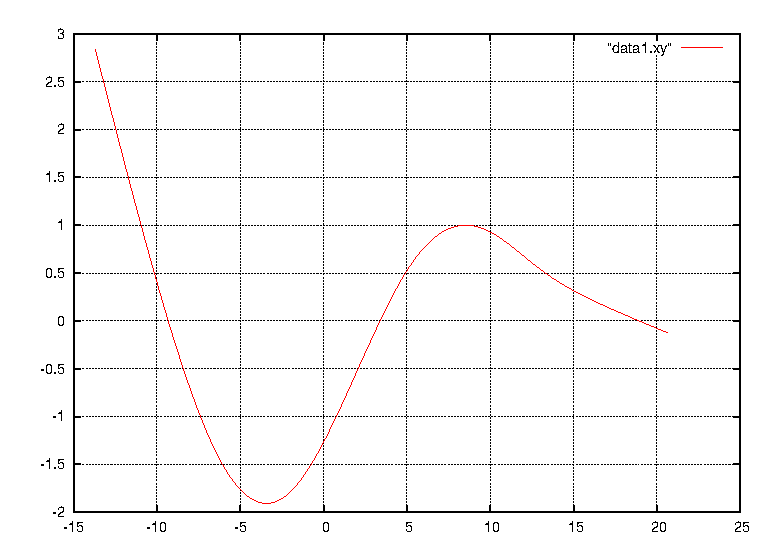
\includegraphics[width=30cm,bb=0 0 696 242]{data1graph.eps}
    \end{figure}

\section{考察}
 スプライン補間した行列(データのX軸とy軸を記した座標)をLU分解することで描画するという構成にかなり時間を労した。なお自作プログラムにはピボットとスケーリングを行ったが、こちらを使った方がスプライン補間したデータを大きい順に並び替えるという点でプログラムを組む上で描画しやすいと思ったためである。

\end{document}
